\section{Context-aware interval transcription}
\label{sec:method}

\begin{figure}[tb]
 \centering
 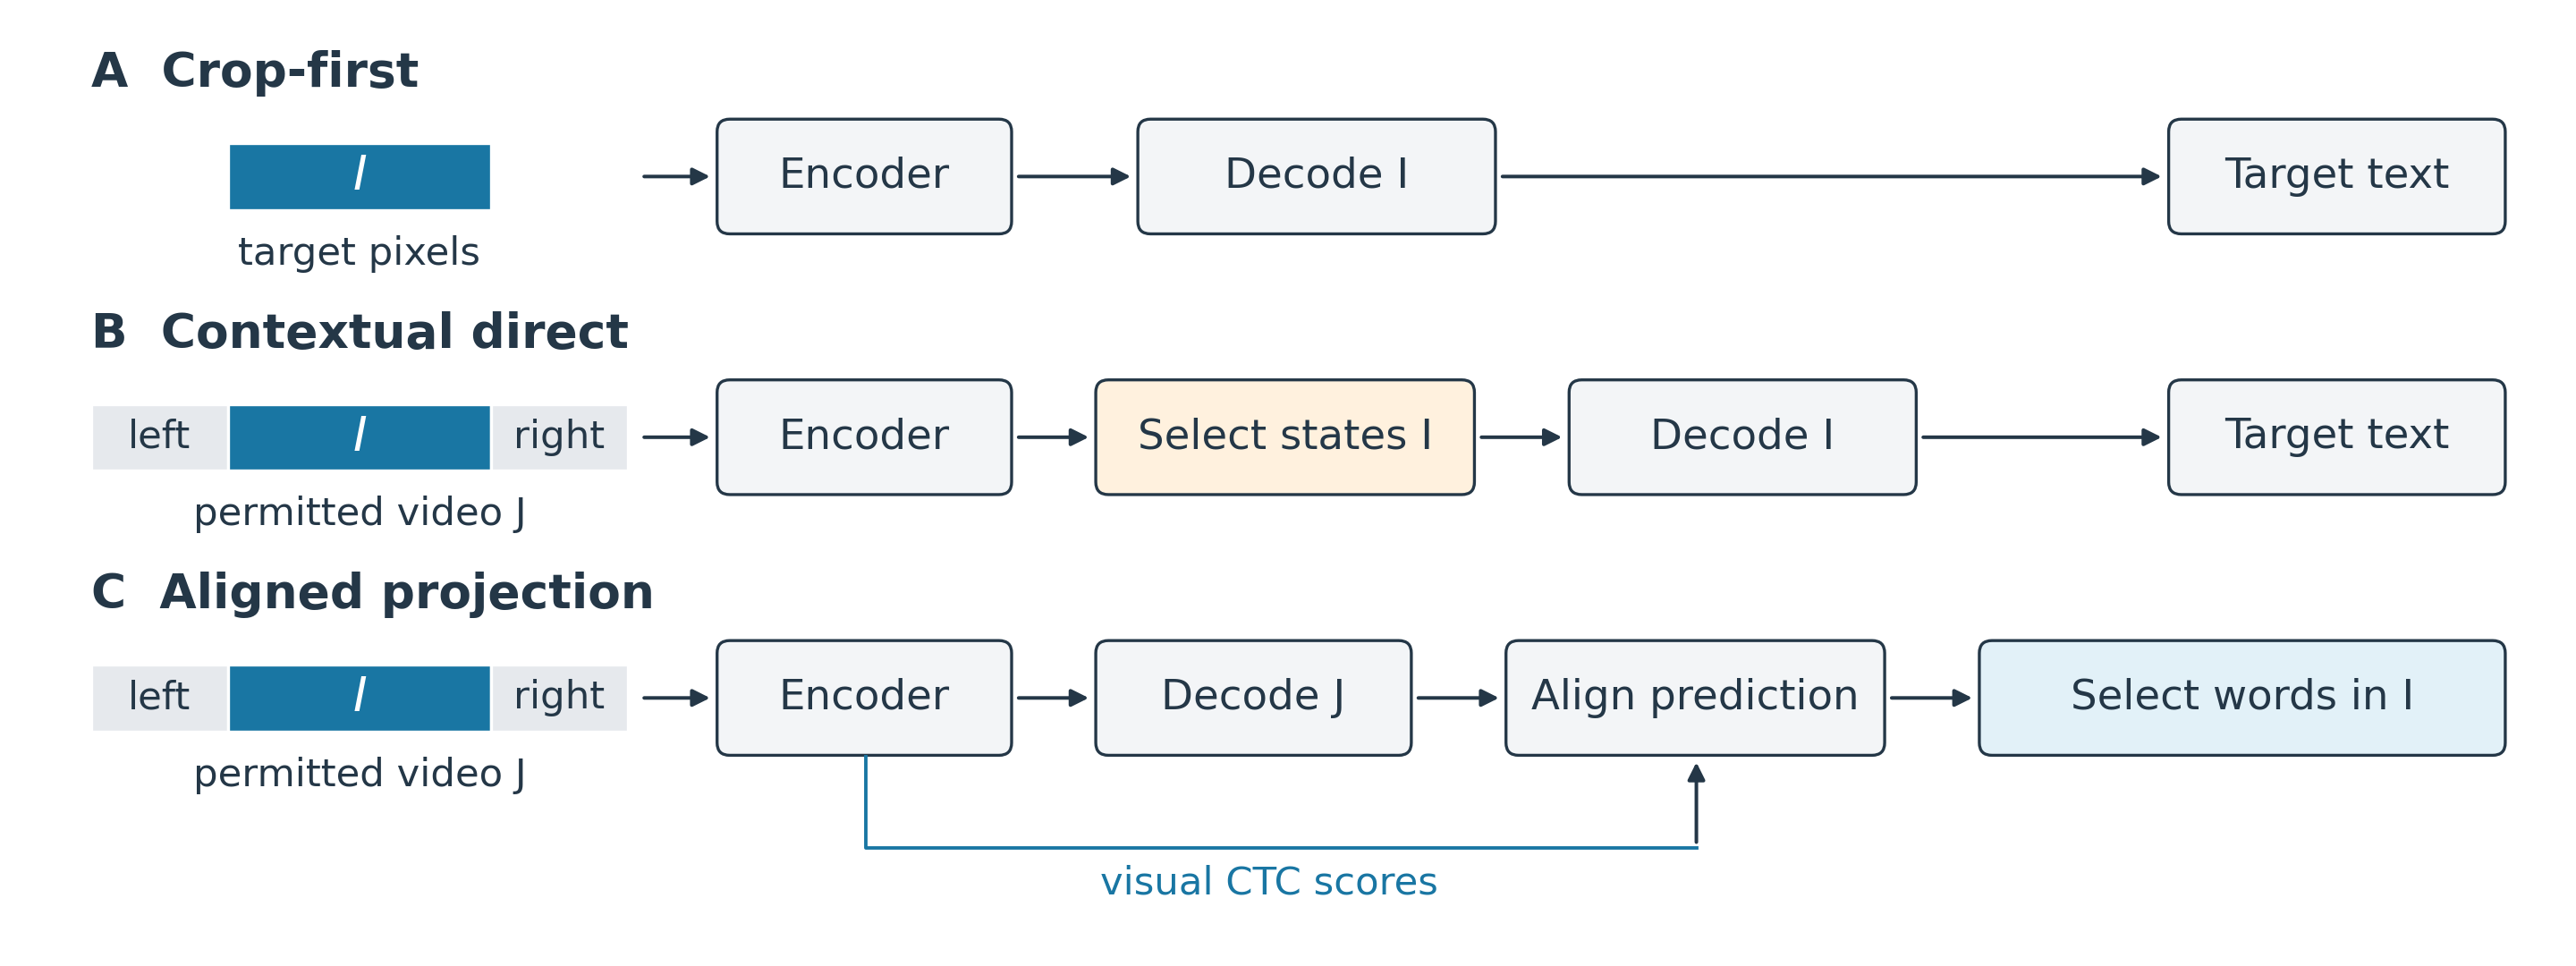
\includegraphics[width=\linewidth]{fig_Interval_Method.png}
 \caption{Three ways to transcribe the same requested interval $I$.
 Crop-first restricts the video before encoding. Contextual direct encodes
 the permitted context $J$ and selects target states before decoding.
 Aligned projection decodes $J$, aligns its own prediction with visual CTC
 scores, and selects words assigned to $I$. B and C observe the same video;
 all alternatives reuse the same frozen recognizer within a corpus.}
 \label{fig:method}
\end{figure}

\subsection{Requested and observed intervals}
Let \(X=(x_0,\ldots,x_{T-1})\) be a prepared mouth-region video, and let
\(I=[a,b)\) be the requested interval in frame coordinates. A context allowance
\((c_{\ell},c_r)\) defines the permitted input
\begin{equation}
 J=[\max(0,a-c_{\ell}),\min(T,b+c_r)).
\end{equation}
The recognizer may observe \(X_J\), while the returned text should belong to
\(I\). Context is real video from the same clip; no frames are fetched beyond its
boundaries. Thus a nominal context budget is an upper bound, and \(J=I\) is
possible for short clips.

Write \(E\) for the visual encoder and \(D\) for a decoder. The encoder also
provides visual CTC token scores \(P_J\). The same pretrained parameters are
used for all inference alternatives within a corpus/model setting.
The experiment distinguishes three operations (Figure~\ref{fig:method}):
\begin{align}
 \widehat{Y}_A &= D(E(X_I)), \label{eq:a}\\
 \widehat{Y}_B &= D\bigl([E(X_J)]_I\bigr), \label{eq:b}\\
 \widehat{Y}_C &= \Pi_I\bigl(D(E(X_J)),P_J\bigr). \label{eq:c}
\end{align}
Crop-first \(A\) restricts pixels before encoding. Contextual direct \(B\)
encodes \(J\), then restricts the decoder to contextual states associated with
\(I\). Projection \(C\) decodes all of \(J\), then restricts the returned words.
Equations~\eqref{eq:b} and~\eqref{eq:c} use the same permitted visual information.
They differ in where the output restriction is applied. The equations motivate
an empirical comparison of state-level and transcript-level readout.

\subsection{Prediction-aligned projection}
The contextual decoder first produces token sequence \(\widehat{z}_J\).
We then align that sequence monotonically to \(P_J\) using a CTC trellis.
Alignment is conditioned on predicted tokens, never on the evaluation
transcript. The recognizer therefore supplies both the text proposal and the
visual scores used to place it.

Tokenizer-aware grouping converts the aligned tokens into complete words.
For a predicted word \(w_k\), the union of its constituent token spans gives
\([s_k,e_k)\) in the contextual input. Its midpoint is mapped back to the
original clip coordinates. Projection returns
\begin{equation}
 \widehat{Y}_C
 = \operatorname{concat}\{w_k:\ a \leq j_0+(s_k+e_k)/2 < b\},
 \label{eq:projection}
\end{equation}
in predicted order, where \(j_0\) is the start of \(J\). Whole words are returned;
the procedure does not cut a subword string at an arbitrary frame.
If the requested interval covers the full available input, the native decoded
transcript is returned directly. This identity case avoids changing ordinary
recognition when there is no outside context.

Projection selects among words in the contextual prediction and preserves
their lexical content and order. It cannot replace a misrecognized word with
the correct word or recover a word omitted by the contextual decoder.
Its role is temporal selection: retaining words assigned to the target and
excluding words assigned outside it. Recognition and temporal assignment thus
jointly determine the returned text. The procedure adds alignment and
allocation work while retaining the pretrained parameters and native CTC head.

\subsection{Controls and unrestricted lookup}
Two allocation controls reuse exactly the same decoded sequence as \(C\).
Uniform-word allocation places its words evenly across \(J\); uniform-token
allocation distributes the predicted tokens evenly and then reconstructs word
spans. Both apply the same midpoint selection rule. Their contrast with \(C\)
isolates the usefulness of predicted visual alignment from the quality of the
generated transcript.

Full-clip lookup \(F\) recognizes \(X\), constructs predicted word times, and
returns words assigned to \(I\). It answers the same target request but has
unrestricted visual input. We also score its complete transcript, as a separate
endpoint, when examining sliding-window recognition. The two endpoints have
different reference denominators and are never treated as interchangeable.

\subsection{Decoder comparability}
We evaluate greedy CTC, pure CTC prefix beam search, and the recognizer's native
hybrid CTC/attention decoding. The pure CTC beam has width 40 and a token-pruning
limit of 64; no external language model is added. Selected-system results use
the decoder chosen for each arm on development data. Matched greedy and pure
CTC results hold that choice fixed across arms.

For hybrid decoding, the output-length cap is derived from the number of
observed frames: \(|I|\) for \(A\), \(|J|\) for \(B/C\), and \(T\) for \(F\).
In particular, \(B\) and \(C\) share the same input-derived cap, although \(B\)
decodes only target states. Greedy and pure CTC use their complete supplied
state sequences rather than an autoregressive cap. Native tokenizer,
normalization, and checkpoint interfaces are retained for each model.

\subsection{Computation across interval requests}
\label{sec:query-computation}
Consider a session with requests \(I_1,\ldots,I_q\), and let
\(\mathcal{J}\) contain their distinct observed intervals. With a fixed
decoder, write \(r(J)\) for recognition cost and \(a(J)\) for the alignment
needed to select words. Ignoring the much smaller selection operation, fresh
projected and full-clip sessions have the respective cost decompositions
\begin{align}
 \tau_C &\simeq \sum_{J\in\mathcal{J}}\bigl[r(J)+a(J)\bigr],\\
 \tau_F &\simeq r([0,T))+a([0,T)).
\end{align}
Alignment is unnecessary when the request covers the entire decoded input.
Exact repeated computations are cached; overlapping but different intervals
are not merged into a shared full-clip encoding. The observed interval set,
rather than the nominal number of requests alone, therefore determines work.
Short clips can make several requested intervals identical.
Distinct targets can also yield the same observed interval after clipping
context at video boundaries. C can then reuse one contextual prediction,
while B may still decode different target-state sequences. Both alternatives
reuse an identical contextual encoding when it is available.

This decomposition links computation to both the observed intervals and their
reuse. B and C encode the same context, while C decodes a larger state sequence
and may require alignment. We measure response cost together with accuracy,
holding the decoder fixed to attribute differences to the inference procedure.
